\documentclass[9pt,ignorenonframetext,xcolor=dvipsnames]{beamer}
\setbeamertemplate{caption}[numbered]
\setbeamertemplate{caption label separator}{: }
\setbeamercolor{caption name}{fg=normal text.fg}
\beamertemplatenavigationsymbolsempty
\usepackage{lmodern}
\usepackage{amssymb,amsmath}
\usepackage{ifxetex,ifluatex}
\usepackage{fixltx2e} % provides \textsubscript
\ifnum 0\ifxetex 1\fi\ifluatex 1\fi=0 % if pdftex
  \usepackage[T1]{fontenc}
  \usepackage[utf8]{inputenc}
\else % if luatex or xelatex
  \ifxetex
    \usepackage{mathspec}
  \else
    \usepackage{fontspec}
  \fi
  \defaultfontfeatures{Ligatures=TeX,Scale=MatchLowercase}
\fi
\usetheme[]{metropolis}
\usefonttheme{serif}
% use upquote if available, for straight quotes in verbatim environments
\IfFileExists{upquote.sty}{\usepackage{upquote}}{}
% use microtype if available
\IfFileExists{microtype.sty}{%
\usepackage{microtype}
\UseMicrotypeSet[protrusion]{basicmath} % disable protrusion for tt fonts
}{}
\newif\ifbibliography
\hypersetup{
            pdftitle={임상연구 설계와 분석을 위한 통계 방법},
            pdfauthor={, Ph.D., Senior researcher},
            colorlinks=true,
            linkcolor=Maroon,
            citecolor=Blue,
            urlcolor=blue,
            breaklinks=true}
\urlstyle{same}  % don't use monospace font for urls

% Prevent slide breaks in the middle of a paragraph:
\widowpenalties 1 10000
\raggedbottom

\AtBeginPart{
  \let\insertpartnumber\relax
  \let\partname\relax
  \frame{\partpage}
}
\AtBeginSection{
  \ifbibliography
  \else
    \let\insertsectionnumber\relax
    \let\sectionname\relax
    \frame{\sectionpage}
  \fi
}
\AtBeginSubsection{
  \let\insertsubsectionnumber\relax
  \let\subsectionname\relax
  \frame{\subsectionpage}
}

\setlength{\parindent}{0pt}
\setlength{\parskip}{6pt plus 2pt minus 1pt}
\setlength{\emergencystretch}{3em}  % prevent overfull lines
\providecommand{\tightlist}{%
  \setlength{\itemsep}{0pt}\setlength{\parskip}{0pt}}
\setcounter{secnumdepth}{0}
\usepackage{kotex}
\usepackage{placeins}
\usepackage{enumerate}
\usepackage{amssymb}
\usepackage{amsmath}
\usepackage{mathtools}
\usepackage{float}
% \usepackage{setspace}\doublespacing
\usepackage{relsize}
\usepackage{bigints}
\usepackage{bm}
\usepackage{booktabs}
\usepackage{dcolumn}
\usepackage{array}
\usepackage[font=footnotesize,labelfont=bf]{caption}
\usepackage{gensymb}
\usepackage{makecell}
\usepackage{graphicx}
\usepackage{rotating}
\usepackage{pgf}
\usepackage{pgfpages}
\usepackage{textpos}
\usepackage{tcolorbox}
\usepackage{lipsum}
\usepackage[framemethod=tikz]{mdframed}

\renewcommand\theadalign{cb}
\renewcommand\theadfont{\bfseries}
\renewcommand\theadgape{\Gape[4pt]}
\renewcommand\cellgape{\Gape[4pt]}
\DeclareMathAlphabet{\mathpzc}{OT1}{pzc}{m}{it}

\renewcommand\theadalign{cb}
\renewcommand\theadfont{\bfseries}
\renewcommand\theadgape{\Gape[4pt]}
\renewcommand\cellgape{\Gape[4pt]}

\newcolumntype{L}[1]{>{\raggedright\let\newline\\
\arraybackslash\hspace{0pt}}m{#1}}
\newcolumntype{C}[1]{>{\centering\let\newline\\
\arraybackslash\hspace{0pt}}m{#1}}
\newcolumntype{R}[1]{>{\raggedleft\let\newline\\
\arraybackslash\hspace{0pt}}m{#1}}
\newcolumntype{P}[1]{>{\raggedright\tabularxbackslash}p{#1}}
\newcommand{\specialcell}[2][c]{%
  \begin{tabular}[#1]{@{}c@{}}#2\end{tabular}}

\setlength\abovecaptionskip{0pt}
\setlength\belowcaptionskip{-5pt}
  
\newlength{\wideitemsep}
\setlength{\wideitemsep}{\itemsep}
\addtolength{\wideitemsep}{0.1cm}
\let\olditem\item
\renewcommand{\item}{\setlength{\itemsep}{\wideitemsep}\olditem}

% \setbeameroption{show notes on second screen=bottom}
\setbeameroption{show notes}
\setbeamertemplate{note page}[plain]
\setbeamertemplate{navigation symbols}{}
\setbeamertemplate{headline}[default]


% \setbeamertemplate{headline}{%
% \leavevmode%
  % \hbox{%
    % \begin{beamercolorbox}[wd=\paperwidth,ht=3ex,dp=1.125ex, right]{palette quaternary}%
    % \usebeamercolor[fg]{navigation symbols}\insertslidenavigationsymbol%
		% \insertframenavigationsymbol%
		% \insertsubsectionnavigationsymbol%
		% \insertsectionnavigationsymbol%
		% \insertdocnavigationsymbol%
		% \insertbackfindforwardnavigationsymbol%
    % \end{beamercolorbox}%
  % }
% }

\addtobeamertemplate{frametitle}{}{
\leavevmode%
  \hbox{%
    \begin{beamercolorbox}[wd=\paperwidth,ht=3ex,dp=1.125ex, right]{palette quaternary}%
    \usebeamercolor[fg]{navigation symbols}\insertslidenavigationsymbol%
		\insertframenavigationsymbol%
		\insertsubsectionnavigationsymbol%
		\insertsectionnavigationsymbol%
		\insertdocnavigationsymbol%
		\insertbackfindforwardnavigationsymbol%
    \end{beamercolorbox}%
  }
}

\setbeamertemplate{footline}
{
  \leavevmode%
  % \includegraphics[width = \paperwidth, height = 0.5cm]{KIOM-BAR.png}
  % \vskip-10pt
  \hbox{%
  \begin{beamercolorbox}[wd=0.3\paperwidth,ht=3ex,dp=1ex,center]{author in head/foot}%
    \usebeamerfont{author in head/foot}{Boncho Ku}
  \end{beamercolorbox}%
  \begin{beamercolorbox}[wd=0.3\paperwidth,ht=3ex,dp=1ex,center]{title in head/foot}%
    \usebeamerfont{title in head/foot}{임상연구 설계와 분석을 위한 통계 방법}
  \end{beamercolorbox}%
  \begin{beamercolorbox}[wd=.4\paperwidth,ht=3ex,dp=1ex,center]{date in head/foot}%
    secondmoon@kiom.re.kr\hspace{0.5cm}\insertframenumber{} / \inserttotalframenumber\hspace*{1ex}
  \end{beamercolorbox}}%
  \vskip0pt%
}

\title{임상연구 설계와 분석을 위한 통계 방법}
\author{\textbf{Boncho Ku}, Ph.D., Senior researcher}
\institute{KM Fundamental Research Division, Korea Institute of Oriental Medicine}
\date{\(16^{\mathrm{th}}\) November, 2017}

\begin{document}
\frame{\titlepage}

\section{\texorpdfstring{Chapter I:
\LARGE{Overview of Statistics}}{Chapter I: }}\label{chapter-i}

\begin{frame}{Famous quotes about statistics}

\begin{mdframed}[backgroundcolor = gray!30]

\textit{There are three types of lies: lies, damn lies, and \textbf{STATISTICS}} (Benjamin Disraeli)

\textit{Fact are stubborn things, but \textbf{STATISTICS} are pliable} (Mark Twain)

and so on ...

\end{mdframed}

Huge number of quotes about statistics commented it in sarcastic tone

\(\rightarrow\) mostly hard to refute

\end{frame}

\begin{frame}{Really?}

\LARGE
\textbf{However ...}

\vspace{0.5cm}

Statistics itself always provides useful information and allows us to
maintain objective perspective based on DATA

\end{frame}

\begin{frame}{What is Statistics?}

\large{So then, what is statistics??}

\vspace{0.5cm}

\begin{columns}
  \begin{column}{0.4\textwidth}
    \begin{center}
      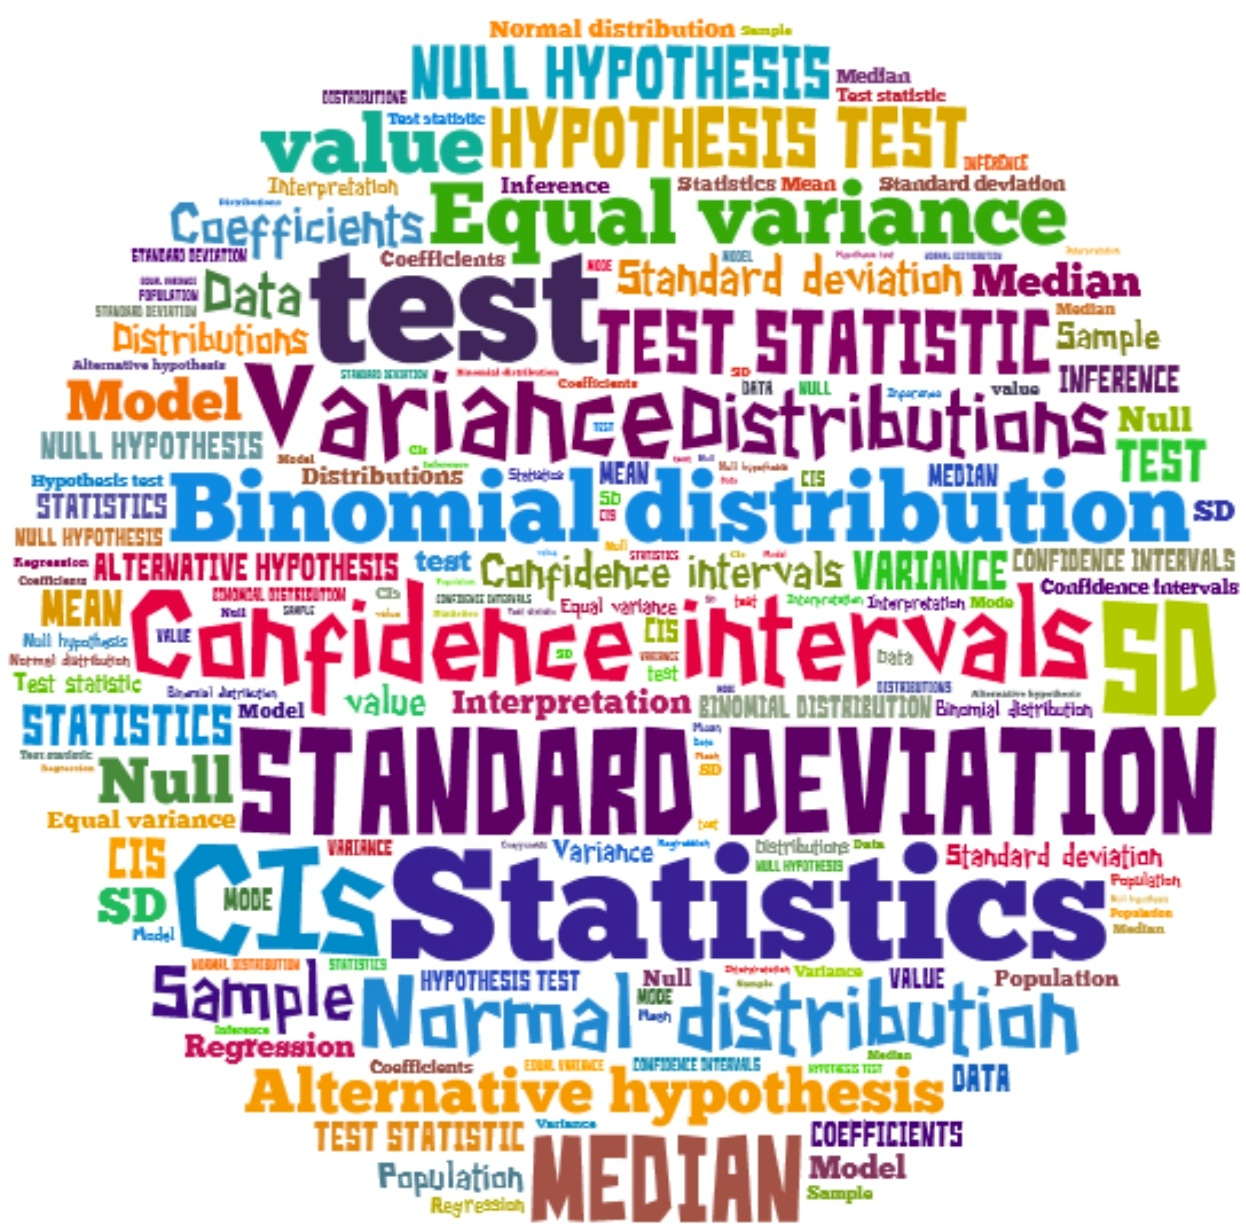
\includegraphics[width = 2.5cm, height = 2.5cm]{StatisticsWords_Meg.jpg}
    \end{center}
  \end{column}
  \begin{column}{0.6\textwidth}
    \begin{center}
      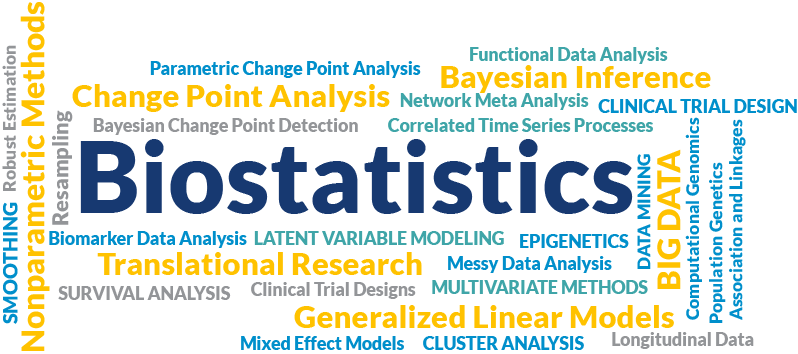
\includegraphics[width = 4.8cm, height = 2.5cm]{wordcloud-biostatics.png}
    \end{center}
  \end{column}
\end{columns}

\tiny{$^{\dagger}$ Each wordcloud was cited from \href{http://blog.trident.edu/-temporary-slug-8756cc7e-1d1b-458e-94e2-3ff603f80c9e}{Trident University International} and \href{http://www.augusta.edu/mcg/dphs/biostats/research/index.php}{Augusta University}, respectively.}

\vspace{0.3cm} \normalsize

\begin{tcolorbox}[colback=gray!10,colframe=black, title=\textbf{Statistics}]
Concerning with \textbf{collection}, \textbf{organization}, \textbf{summarization} and \textbf{analysis} of \textbf{DATA}
\end{tcolorbox}

\end{frame}

\begin{frame}{Main Pillars of Statistics}

\LARGE

\begin{block}{The most important things in statistics}

\normalsize

\begin{enumerate}
\def\labelenumi{\arabic{enumi}.}
\tightlist
\item
  Data (sample)

  \begin{itemize}
  \tightlist
  \item
    Investigation, experiment, and survey
  \item
    Gathering numbers (for quantitative analysis)
  \end{itemize}
\item
  Description or Summarization

  \begin{itemize}
  \tightlist
  \item
    Table, chart, and so on
  \item
    Based on summarized statistics (e.g.~mean, standard deviation,
    median, \ldots{})
  \end{itemize}
\item
  Inference

  \begin{itemize}
  \tightlist
  \item
    Numerous statistical tests and models based on probability theory
  \item
    e.g.~two-sample t-test, ANOVA, ANCOVA, regression, and so on
  \end{itemize}
\end{enumerate}

\end{block}

\end{frame}

\begin{frame}{Why should we collect data (sample)?}

\begin{block}{Measure everything from POPULATION}

\begin{itemize}
\tightlist
\item
  Benefits

  \begin{itemize}
  \tightlist
  \item
    You will get exactly correct answer
  \item
    No need to meet an awkward statistician LIKE ME
  \end{itemize}
\item
  If you had a plenty of

  \begin{itemize}
  \tightlist
  \item
    Money (typing ``SHOW ME THE MONEY'' may help your budget)
  \item
    Time (TOO SHORT TO COLLECT data of entire population)
  \end{itemize}
\end{itemize}

\end{block}

\begin{block}{Inferential approach based on SAMPLE}

\begin{itemize}
\tightlist
\item
  If we have a proper sample that represents the whole population, you
  can get NEARLY the correct answer
\item
  Estimation and hypothesis testing
\end{itemize}

\end{block}

\end{frame}

\begin{frame}{Parameter vs.~Estimates}

\begin{block}{Parameter}

Parameters exist somewhere in the universe \(\rightarrow\) the true
value representing the target population

From the view of \textit{frequentist},

\begin{itemize}
\tightlist
\item
  Parameters are fixed \(\rightarrow\) never changing
\item
  Parameters exists but we never know the true value of them
\item
  But we can ``guess'' them from sample
\end{itemize}

\end{block}

\end{frame}

\begin{frame}{Parameter vs.~Estimates}

\begin{block}{Estimates}

\begin{itemize}
\tightlist
\item
  Estimating parameters based on the given samples (data)
\item
  Estimates have a variation in accordance with different samples or
  data
\end{itemize}

\begin{mdframed}[backgroundcolor = gray!30]

The data is an aspect of the real world we have captured

\end{mdframed}

\begin{itemize}
\tightlist
\item
  How good is our estimation?

  \begin{itemize}
  \tightlist
  \item
    Estimation inevitably involves \textbf{ERROR}
  \item
    Error measures: standard error (SE) \(\rightarrow\) reliability of
    an estimate
  \end{itemize}
\end{itemize}

\[
  \mathrm{SE} = \frac{\sigma}{\sqrt{N}}
\]

\begin{mdframed}[backgroundcolor = gray!30]
\textbf{\textit{Measurement is ubiquitous $\rightarrow$ then error is also ubiquitous.}}
\end{mdframed}

\end{block}

\end{frame}

\begin{frame}{Type of variables}

\textbf{Data consist of a set of independent sample and measured variables}

\begin{table}
  \centering
  \caption{Types of variable based on their scales}
  \begingroup\footnotesize
  \begin{tabular}{lp{12em}p{8em}}
    \toprule
  \textbf{Scale}  &  \textbf{Example}                                                & \textbf{Operation} \\
    \midrule 
  \multicolumn{3}{L{5cm}}{\textbf{Qualitative (질적변수)}} \\
  \hspace{2.5mm} Nominal (명목)  & sex, marital status, blood type, race, eye colour, religion, ... & counting          \\ 
  \hspace{2.5mm} Ordinal (순서)  & grade, education level, preference, severity, ...                & counting, ranking \\
  \multicolumn{3}{L{5cm}}{\textbf{Quantitative (양적변수)}} \\
  \hspace{2.5mm} Interval (구간) & temperature, IQ, SAT score, ...                                  & counting, ranking, $+$, $-$ \\
  \hspace{2.5mm} Ratio (비율)    & distance, length, height, weight, BMI, blood pressure, ...       & counting, ranking, $+$, $-$, $\times$, $\div$ \\
  \bottomrule
  \end{tabular}
  \endgroup
\end{table}

\end{frame}

\begin{frame}{Can we separate types of variable clearly?}

Continuous variable is limited by the precision of the measurement

\begin{block}{Example}

\begin{itemize}
\tightlist
\item
  Height: measured to the nearest centimeter \(\rightarrow\) continuous
  variable?
\item
  Age: measured to the year but theoretically, measured to any level of
  precision (e.g.~month, day, and time)
\end{itemize}

\begin{mdframed}[backgroundcolor = gray!30]
In practice, all variables are discrete but some variables can be treated as continuous when its distribution can be well approximated by a continuous distribution.
\end{mdframed}

\end{block}

\end{frame}

\begin{frame}{How to express your data?}

\begin{mdframed}[backgroundcolor = gray!30]
Data themselves are just a bunch of numbers $\rightarrow$ how to extract meaningful information from data?
\end{mdframed}

\begin{block}{Descriptive statistics}

\begin{itemize}
\tightlist
\item
  Summary statistics: all information of data are represented by a
  certain type of numbers

  \begin{itemize}
  \tightlist
  \item
    Example: mean, median, proportion, standard deviation, interquartile
    range, percentile, \ldots{} \(\rightarrow\) developing
    ``\textit{statphobia}''
  \end{itemize}
\end{itemize}

\begin{table}[H]
\centering
\caption{Descriptive statistics of ``mpg'' dataset} 
\label{tab:demo-1}
\begingroup\footnotesize
\begin{tabular}{lrrrrrrrrr}
 \textbf{Variable} & $\mathbf{n}$ & \textbf{Min} & $\mathbf{q_1}$ & $\mathbf{\widetilde{x}}$ & $\mathbf{\bar{x}}$ & $\mathbf{q_3}$ & \textbf{Max} & $\mathbf{s}$ & \textbf{IQR} \\ 
  \hline
displ & 234 &    1.6 &    2.4 &    3.3 &    3.5 &    4.6 &    7 & 1.3 & 2.2 \\ 
  year & 234 & 1999.0 & 1999.0 & 2003.5 & 2003.5 & 2008.0 & 2008 & 4.5 & 9.0 \\ 
  cyl & 234 &    4.0 &    4.0 &    6.0 &    5.9 &    8.0 &    8 & 1.6 & 4.0 \\ 
  cty & 234 &    9.0 &   14.0 &   17.0 &   16.9 &   19.0 &   35 & 4.3 & 5.0 \\ 
  hwy & 234 &   12.0 &   18.0 &   24.0 &   23.4 &   27.0 &   44 & 6.0 & 9.0 \\ 
  \end{tabular}
\endgroup
\end{table}

\end{block}

\end{frame}

\begin{frame}{How to express your data?}

\begin{block}{Example of polar area diagram by Florence Nightingale
(1820 \(\sim\) 1910)}

\begin{center}
  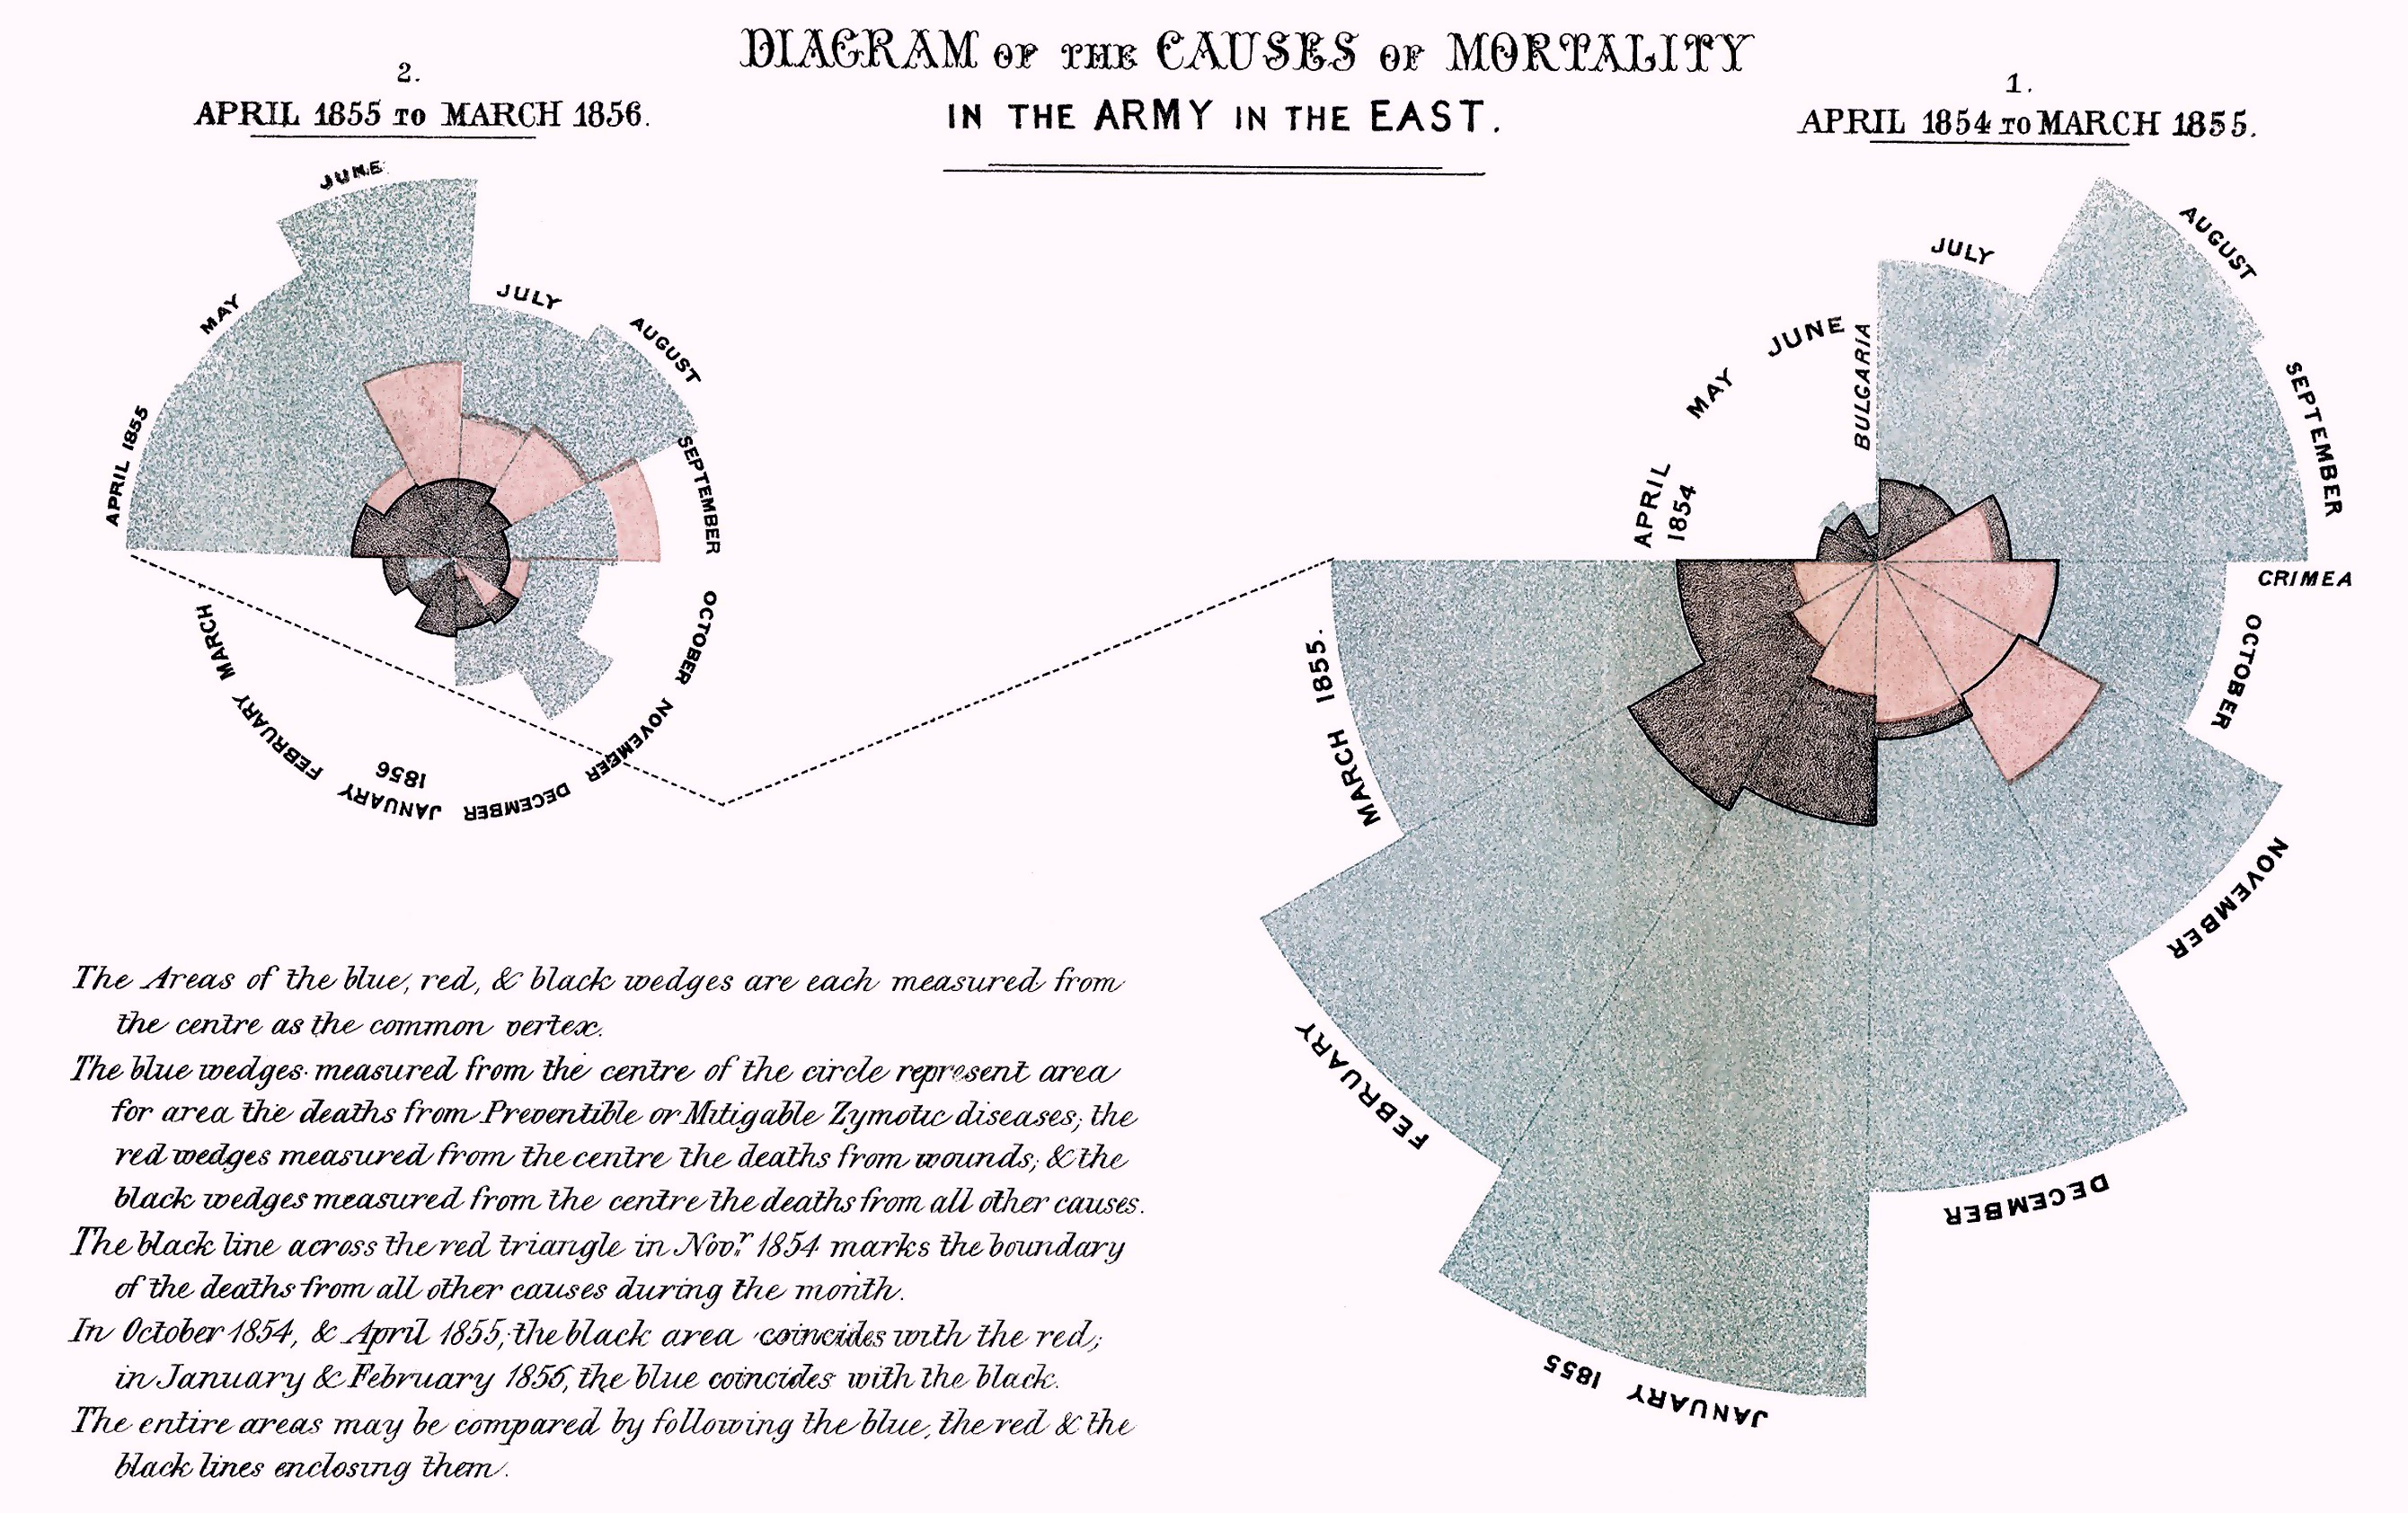
\includegraphics[width = 10cm, height = 6cm]{Nightingale-mortality.jpg}
\end{center}

\end{block}

\end{frame}

\begin{frame}{How to express your data?}

\begin{block}{Example of data visualization}

\begin{figure}[H]

{\centering 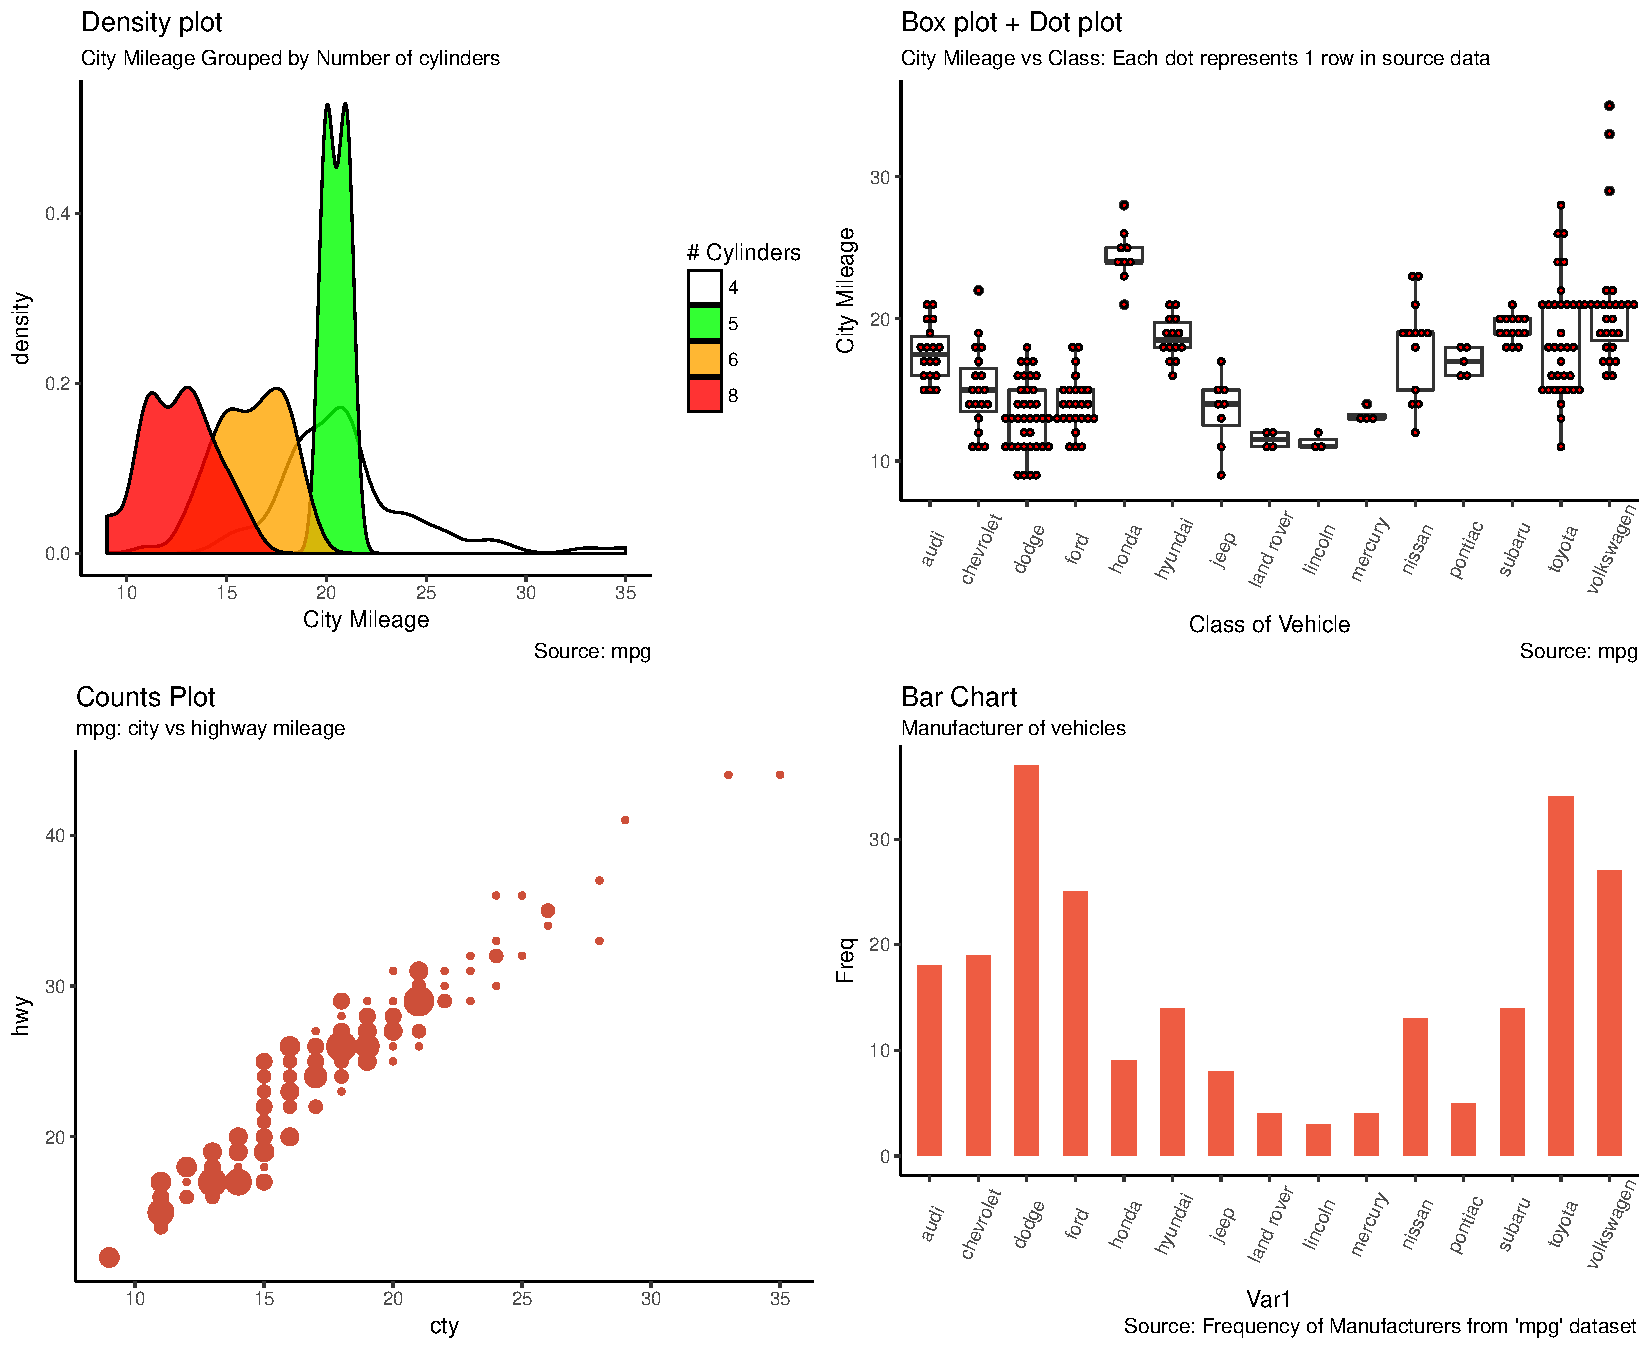
\includegraphics[width=8cm,height=6cm]{Figures/mpg-example-1} 

}

\caption{Data visualization examples for ``mpg'' dataset. All plots are available at http://r-statistics.co/Top50-Ggplot2-Visualizations-MasterList-R-Code.html}\label{fig:mpg-example}
\end{figure}

\end{block}

\end{frame}

\begin{frame}{How to express your data?}

\begin{block}{Data visualization}

\begin{mdframed}[backgroundcolor = gray!30]
Sometimes, a graph provides us more useful information than complex tables
\end{mdframed}

\end{block}

\begin{block}{Various types of statistical graphs}

\begin{itemize}
\tightlist
\item
  Histogram, boxplot, Q-Q plot, scatterplot, \ldots{}
\item
  Do NOT rely only on NUMBERS, Do draw a PLOT!!
\end{itemize}

\end{block}

\end{frame}

\begin{frame}{Is description of data fully enough?}

Again, data are the small aspect of the real world.

Statistical inference provides us more reasonable interpretation
regarding to the uncertainty of data.

\begin{tcolorbox}[colback=gray!10,colframe=black, title=\textbf{Two main category of statistical inference}]
\begin{itemize}
  \item \textbf{Estimation}
  \item \textbf{Hypothesis testing}
\end{itemize}
\end{tcolorbox}

\end{frame}

\begin{frame}{Meaning of 95\% confidence interval}

\begin{figure}[H]

{\centering \includegraphics[width=10cm,height=5cm]{Figures/unnamed-chunk-1-1} 

}

\caption{95\% confidence intervals for 100 independent drawn samples with $n = 100$.}\label{fig:unnamed-chunk-1}
\end{figure}

\end{frame}

\section{Clinical Research}\label{clinical-research}

\begin{frame}{Overview}

\LARGE{\textbf{Research or trial?}}

\begin{block}{Research}

\normalsize{자료의 수집과 분석 목적이 학술적 목적에 국한된 모든 종류의 연구 및 실험}

\end{block}

\begin{block}{Trial}

\normalsize{자료의 수집과 분석 목적이 이윤추구 또는 허가에 목적이 있는 임상시험}

\end{block}

\end{frame}

\begin{frame}{Observational Study}

\begin{block}{Cross-sectional study (단면적 관찰연구)}

\begin{enumerate}
\def\labelenumi{\arabic{enumi}.}
\tightlist
\item
  prevalence study
\item
  Diagostic test
\item
  Ecological study
\item
  Validity, Reliability, and agreement study
\end{enumerate}

\end{block}

\begin{block}{Longitudinal study (종단적 관찰연구)}

\begin{enumerate}
\def\labelenumi{\arabic{enumi}.}
\tightlist
\item
  Prospective study
\item
  Retrospective study
\end{enumerate}

\end{block}

\end{frame}

\begin{frame}{Experimental Study}

\begin{block}{Randomized controlled trial}

\end{block}

\begin{block}{Pilot study}

\end{block}

\begin{block}{Exploratory study}

\end{block}

\begin{block}{Confirmative study}

\end{block}

\end{frame}

\section{Type of outcome variables}\label{type-of-outcome-variables}

\begin{frame}{Primary outcomes}

\end{frame}

\begin{frame}{Secondary outcomes}

\end{frame}

\begin{frame}{Surrogate variables}

\end{frame}

\begin{frame}{Global assessment variable}

\end{frame}

\section{Sample size calculation}\label{sample-size-calculation}

\begin{frame}{Overview}

\begin{block}{Two approaches}

\begin{enumerate}
\def\labelenumi{\arabic{enumi}.}
\tightlist
\item
  Based on the marginal error rate \(\rightarrow\) population based
  observational study
\item
  Based on the effectiveness between concerning groups \(\rightarrow\)
  experimental study
\end{enumerate}

\textbf{Both approaches are based on previous studies}

\textbf{Is your study entirely new?}

\end{block}

\end{frame}

\begin{frame}{Observational study}

\end{frame}

\begin{frame}{Observational study: prevalence study}

\end{frame}

\begin{frame}{Observational study: prevalence study}

\end{frame}

\begin{frame}{Parallel design}

\end{frame}

\begin{frame}{\(2\times 2\) cross-over design}

\end{frame}

\begin{frame}{Factorial design}

\end{frame}

\section{Multiple comparison}\label{multiple-comparison}

\begin{frame}{What makes data significant?}

\begin{enumerate}
\def\labelenumi{\arabic{enumi}.}
\tightlist
\item
  Data themselves contain unexpected errors
\item
  Bias
\item
  Just conincidence
\item
  Our hypothesis is working
\end{enumerate}

\end{frame}

\begin{frame}{Torturing data}

\end{frame}

\section{Statistical Analysis}\label{statistical-analysis}

\begin{frame}{Overview}

\end{frame}

\begin{frame}{Independent two sample t-test}

\begin{enumerate}
\def\labelenumi{\arabic{enumi}.}
\tightlist
\item
  Too easy, but very useful methodology for the comparison of sample
  means between two groups
\end{enumerate}

\end{frame}

\begin{frame}{Analysis of Variance (ANOVA)}

\end{frame}

\begin{frame}{Analysis of Covariance (ANCOVA)}

\end{frame}

\begin{frame}{Simple or multiple regression}

\end{frame}

\begin{frame}{Repeated Measures ANOVA}

\end{frame}

\begin{frame}{Linear mixed effects model}

\end{frame}

\begin{frame}{Reliability analysis}

\begin{block}{Cohen's \(\kappa\)}

\end{block}

\begin{block}{Cronbach's \(\alpha\)}

\end{block}

\begin{block}{Intra Class Correlation (ICC)}

\end{block}

\end{frame}

\end{document}
